\documentclass[twoside]{book}

% Packages required by doxygen
\usepackage{fixltx2e}
\usepackage{calc}
\usepackage{doxygen}
\usepackage[export]{adjustbox} % also loads graphicx
\usepackage{graphicx}
\usepackage[utf8]{inputenc}
\usepackage{makeidx}
\usepackage{multicol}
\usepackage{multirow}
\PassOptionsToPackage{warn}{textcomp}
\usepackage{textcomp}
\usepackage[nointegrals]{wasysym}
\usepackage[table]{xcolor}

% Font selection
\usepackage[T1]{fontenc}
\usepackage[scaled=.90]{helvet}
\usepackage{courier}
\usepackage{amssymb}
\usepackage{sectsty}
\renewcommand{\familydefault}{\sfdefault}
\allsectionsfont{%
  \fontseries{bc}\selectfont%
  \color{darkgray}%
}
\renewcommand{\DoxyLabelFont}{%
  \fontseries{bc}\selectfont%
  \color{darkgray}%
}
\newcommand{\+}{\discretionary{\mbox{\scriptsize$\hookleftarrow$}}{}{}}

% Page & text layout
\usepackage{geometry}
\geometry{%
  a4paper,%
  top=2.5cm,%
  bottom=2.5cm,%
  left=2.5cm,%
  right=2.5cm%
}
\tolerance=750
\hfuzz=15pt
\hbadness=750
\setlength{\emergencystretch}{15pt}
\setlength{\parindent}{0cm}
\setlength{\parskip}{3ex plus 2ex minus 2ex}
\makeatletter
\renewcommand{\paragraph}{%
  \@startsection{paragraph}{4}{0ex}{-1.0ex}{1.0ex}{%
    \normalfont\normalsize\bfseries\SS@parafont%
  }%
}
\renewcommand{\subparagraph}{%
  \@startsection{subparagraph}{5}{0ex}{-1.0ex}{1.0ex}{%
    \normalfont\normalsize\bfseries\SS@subparafont%
  }%
}
\makeatother

% Headers & footers
\usepackage{fancyhdr}
\pagestyle{fancyplain}
\fancyhead[LE]{\fancyplain{}{\bfseries\thepage}}
\fancyhead[CE]{\fancyplain{}{}}
\fancyhead[RE]{\fancyplain{}{\bfseries\leftmark}}
\fancyhead[LO]{\fancyplain{}{\bfseries\rightmark}}
\fancyhead[CO]{\fancyplain{}{}}
\fancyhead[RO]{\fancyplain{}{\bfseries\thepage}}
\fancyfoot[LE]{\fancyplain{}{}}
\fancyfoot[CE]{\fancyplain{}{}}
\fancyfoot[RE]{\fancyplain{}{\bfseries\scriptsize Generated by Doxygen }}
\fancyfoot[LO]{\fancyplain{}{\bfseries\scriptsize Generated by Doxygen }}
\fancyfoot[CO]{\fancyplain{}{}}
\fancyfoot[RO]{\fancyplain{}{}}
\renewcommand{\footrulewidth}{0.4pt}
\renewcommand{\chaptermark}[1]{%
  \markboth{#1}{}%
}
\renewcommand{\sectionmark}[1]{%
  \markright{\thesection\ #1}%
}

% Indices & bibliography
\usepackage{natbib}
\usepackage[titles]{tocloft}
\setcounter{tocdepth}{3}
\setcounter{secnumdepth}{5}
\makeindex

% Hyperlinks (required, but should be loaded last)
\usepackage{ifpdf}
\ifpdf
  \usepackage[pdftex,pagebackref=true]{hyperref}
\else
  \usepackage[ps2pdf,pagebackref=true]{hyperref}
\fi
\hypersetup{%
  colorlinks=true,%
  linkcolor=blue,%
  citecolor=blue,%
  unicode%
}

% Custom commands
\newcommand{\clearemptydoublepage}{%
  \newpage{\pagestyle{empty}\cleardoublepage}%
}

\usepackage{caption}
\captionsetup{labelsep=space,justification=centering,font={bf},singlelinecheck=off,skip=4pt,position=top}

%===== C O N T E N T S =====

\begin{document}

% Titlepage & ToC
\hypersetup{pageanchor=false,
             bookmarksnumbered=true,
             pdfencoding=unicode
            }
\pagenumbering{alph}
\begin{titlepage}
\vspace*{7cm}
\begin{center}%
{\Large H\+I\+D\+L\+CD }\\
\vspace*{1cm}
{\large Generated by Doxygen 1.8.13}\\
\end{center}
\end{titlepage}
\clearemptydoublepage
\pagenumbering{roman}
\tableofcontents
\clearemptydoublepage
\pagenumbering{arabic}
\hypersetup{pageanchor=true}

%--- Begin generated contents ---
\chapter{H\+I\+D\+L\+CD Driver library for H\+I\+D-\/compliant L\+CD Display}
\label{index}\hypertarget{index}{}This driver allows the host to communicate with H\+I\+D-\/compliant Auxiliary Display based on Arduino.\+The main idea of this library is to provide a simple unified communication with the small L\+CD displays supported by Arduino. Such displays can be used for showing system information such as hardware temperature, fan speed, percentage of memory available etc., and used by host applications as necessary. H\+I\+D\+L\+CD is build on top of the H\+I\+D\+A\+PI library and provides the next level of abstraction specific to the H\+I\+D-\/compliant auxiliary L\+CD displays.

\hyperlink{group__API}{H\+ID A\+PI} 
\chapter{Module Index}
\section{Modules}
Here is a list of all modules\+:\begin{DoxyCompactList}
\item \contentsline{section}{H\+ID A\+PI}{\pageref{group__API}}{}
\end{DoxyCompactList}

\chapter{Class Index}
\section{Class List}
Here are the classes, structs, unions and interfaces with brief descriptions\+:\begin{DoxyCompactList}
\item\contentsline{section}{\hyperlink{structHIDDisplayParams}{H\+I\+D\+Display\+Params} \\*The structure holding the physical parameters and other capabilities of the L\+CD display }{\pageref{structHIDDisplayParams}}{}
\end{DoxyCompactList}

\chapter{File Index}
\section{File List}
Here is a list of all documented files with brief descriptions\+:\begin{DoxyCompactList}
\item\contentsline{section}{hidlcd/\hyperlink{hidlcd_8h}{hidlcd.\+h} }{\pageref{hidlcd_8h}}{}
\end{DoxyCompactList}

\chapter{Module Documentation}
\hypertarget{group__API}{}\section{H\+ID A\+PI}
\label{group__API}\index{H\+I\+D A\+PI@{H\+I\+D A\+PI}}
\subsection*{Functions}
\begin{DoxyCompactItemize}
\item 
\hyperlink{structHIDDisplayParams}{H\+I\+D\+Display\+Params} $\ast$H\+I\+D\+\_\+\+A\+P\+I\+\_\+\+E\+X\+P\+O\+RT H\+I\+D\+\_\+\+A\+P\+I\+\_\+\+C\+A\+LL \hyperlink{group__API_gabb41034a653433cec87bd56d20e7da32}{hidlcd\+\_\+get\+\_\+display\+\_\+params} (hid\+\_\+device $\ast$dev)
\begin{DoxyCompactList}\small\item\em Returns the physical parameters of the connected auxiliary L\+CD display. \end{DoxyCompactList}\item 
H\+I\+D\+\_\+\+A\+P\+I\+\_\+\+E\+X\+P\+O\+RT hid\+\_\+device $\ast$H\+I\+D\+\_\+\+A\+P\+I\+\_\+\+C\+A\+LL \hyperlink{group__API_ga9fbc6a6acff713baca89139cc99fed1e}{hidlcd\+\_\+open} (unsigned short vendor\+\_\+id, unsigned short product\+\_\+id, const wchar\+\_\+t $\ast$serial\+\_\+number)
\begin{DoxyCompactList}\small\item\em Returns the device handle. \end{DoxyCompactList}\item 
void H\+I\+D\+\_\+\+A\+P\+I\+\_\+\+E\+X\+P\+O\+RT H\+I\+D\+\_\+\+A\+P\+I\+\_\+\+C\+A\+LL \hyperlink{group__API_gab5076b4a075677b9298c2261621668bf}{hidlcd\+\_\+close} (hid\+\_\+device $\ast$dev)
\begin{DoxyCompactList}\small\item\em Closes the device handle and releases associated resources. \end{DoxyCompactList}\item 
int H\+I\+D\+\_\+\+A\+P\+I\+\_\+\+E\+X\+P\+O\+RT H\+I\+D\+\_\+\+A\+P\+I\+\_\+\+C\+A\+LL \hyperlink{group__API_ga67748e0754a894b7d04d9f0beef058fc}{hidlcd\+\_\+exit} (void)
\begin{DoxyCompactList}\small\item\em Closes the H\+I\+D\+L\+CD library and releases associated resources. \end{DoxyCompactList}\item 
int H\+I\+D\+\_\+\+A\+P\+I\+\_\+\+E\+X\+P\+O\+RT H\+I\+D\+\_\+\+A\+P\+I\+\_\+\+C\+A\+LL \hyperlink{group__API_ga37c732d4d14ea4584ee33e6e258deba7}{hidlcd\+\_\+init} (void)
\begin{DoxyCompactList}\small\item\em Initialize the H\+I\+D\+L\+CD library. \end{DoxyCompactList}\item 
int H\+I\+D\+\_\+\+A\+P\+I\+\_\+\+E\+X\+P\+O\+RT H\+I\+D\+\_\+\+A\+P\+I\+\_\+\+C\+A\+LL \hyperlink{group__API_ga0c27c33eef05230a5ed6e1d6ea6cb489}{hidlcd\+\_\+set\+\_\+cursor} (hid\+\_\+device $\ast$dev, u\+\_\+int8\+\_\+t row, u\+\_\+int8\+\_\+t col)
\begin{DoxyCompactList}\small\item\em This function sets the cursor of the L\+CD display in the specified position. \end{DoxyCompactList}\item 
int H\+I\+D\+\_\+\+A\+P\+I\+\_\+\+E\+X\+P\+O\+RT H\+I\+D\+\_\+\+A\+P\+I\+\_\+\+C\+A\+LL \hyperlink{group__API_gae33cb27bbbe1ae372fd3b98f16bd665d}{hidlcd\+\_\+set\+\_\+cursor\+\_\+flags\+\_\+ext} (hid\+\_\+device $\ast$dev, u\+\_\+int8\+\_\+t flags, u\+\_\+int8\+\_\+t mode)
\begin{DoxyCompactList}\small\item\em This function sets the cursor extended parameters and display mode. \end{DoxyCompactList}\item 
int H\+I\+D\+\_\+\+A\+P\+I\+\_\+\+E\+X\+P\+O\+RT H\+I\+D\+\_\+\+A\+P\+I\+\_\+\+C\+A\+LL \hyperlink{group__API_gab5c3e5de5b25ce048739fb5570fceabc}{hidlcd\+\_\+print} (hid\+\_\+device $\ast$dev, \hyperlink{structHIDDisplayParams}{H\+I\+D\+Display\+Params} $\ast$display\+\_\+params, const char $\ast$string)
\begin{DoxyCompactList}\small\item\em Prints the text on the L\+CD screen. \end{DoxyCompactList}\item 
int H\+I\+D\+\_\+\+A\+P\+I\+\_\+\+E\+X\+P\+O\+RT H\+I\+D\+\_\+\+A\+P\+I\+\_\+\+C\+A\+LL \hyperlink{group__API_gad6c000babbc378230a1a7023bd53b8b2}{hidlcd\+\_\+send\+\_\+command\+\_\+ext} (hid\+\_\+device $\ast$dev, u\+\_\+int8\+\_\+t command, u\+\_\+int8\+\_\+t mode)
\begin{DoxyCompactList}\small\item\em Sends the command to the L\+CD display with mode. \end{DoxyCompactList}\item 
int H\+I\+D\+\_\+\+A\+P\+I\+\_\+\+E\+X\+P\+O\+RT H\+I\+D\+\_\+\+A\+P\+I\+\_\+\+C\+A\+LL \hyperlink{group__API_ga1ec7653ee073e917475c01ee9e1252e4}{hidlcd\+\_\+send\+\_\+command} (hid\+\_\+device $\ast$dev, u\+\_\+int8\+\_\+t command)
\begin{DoxyCompactList}\small\item\em Sends the command to the L\+CD display. \end{DoxyCompactList}\end{DoxyCompactItemize}


\subsection{Detailed Description}


\subsection{Function Documentation}
\mbox{\Hypertarget{group__API_gab5076b4a075677b9298c2261621668bf}\label{group__API_gab5076b4a075677b9298c2261621668bf}} 
\index{H\+I\+D A\+PI@{H\+I\+D A\+PI}!hidlcd\+\_\+close@{hidlcd\+\_\+close}}
\index{hidlcd\+\_\+close@{hidlcd\+\_\+close}!H\+I\+D A\+PI@{H\+I\+D A\+PI}}
\subsubsection{\texorpdfstring{hidlcd\+\_\+close()}{hidlcd\_close()}}
{\footnotesize\ttfamily void H\+I\+D\+\_\+\+A\+P\+I\+\_\+\+E\+X\+P\+O\+RT H\+I\+D\+\_\+\+A\+P\+I\+\_\+\+C\+A\+LL hidlcd\+\_\+close (\begin{DoxyParamCaption}\item[{hid\+\_\+device $\ast$}]{dev }\end{DoxyParamCaption})}



Closes the device handle and releases associated resources. 


\begin{DoxyParams}{Parameters}
{\em dev} & A device handle returned from hid\+\_\+open(). \\
\hline
\end{DoxyParams}
\mbox{\Hypertarget{group__API_ga67748e0754a894b7d04d9f0beef058fc}\label{group__API_ga67748e0754a894b7d04d9f0beef058fc}} 
\index{H\+I\+D A\+PI@{H\+I\+D A\+PI}!hidlcd\+\_\+exit@{hidlcd\+\_\+exit}}
\index{hidlcd\+\_\+exit@{hidlcd\+\_\+exit}!H\+I\+D A\+PI@{H\+I\+D A\+PI}}
\subsubsection{\texorpdfstring{hidlcd\+\_\+exit()}{hidlcd\_exit()}}
{\footnotesize\ttfamily int H\+I\+D\+\_\+\+A\+P\+I\+\_\+\+E\+X\+P\+O\+RT H\+I\+D\+\_\+\+A\+P\+I\+\_\+\+C\+A\+LL hidlcd\+\_\+exit (\begin{DoxyParamCaption}\item[{void}]{ }\end{DoxyParamCaption})}



Closes the H\+I\+D\+L\+CD library and releases associated resources. 

\begin{DoxyReturn}{Returns}

\end{DoxyReturn}
\mbox{\Hypertarget{group__API_gabb41034a653433cec87bd56d20e7da32}\label{group__API_gabb41034a653433cec87bd56d20e7da32}} 
\index{H\+I\+D A\+PI@{H\+I\+D A\+PI}!hidlcd\+\_\+get\+\_\+display\+\_\+params@{hidlcd\+\_\+get\+\_\+display\+\_\+params}}
\index{hidlcd\+\_\+get\+\_\+display\+\_\+params@{hidlcd\+\_\+get\+\_\+display\+\_\+params}!H\+I\+D A\+PI@{H\+I\+D A\+PI}}
\subsubsection{\texorpdfstring{hidlcd\+\_\+get\+\_\+display\+\_\+params()}{hidlcd\_get\_display\_params()}}
{\footnotesize\ttfamily \hyperlink{structHIDDisplayParams}{H\+I\+D\+Display\+Params}$\ast$ H\+I\+D\+\_\+\+A\+P\+I\+\_\+\+E\+X\+P\+O\+RT H\+I\+D\+\_\+\+A\+P\+I\+\_\+\+C\+A\+LL hidlcd\+\_\+get\+\_\+display\+\_\+params (\begin{DoxyParamCaption}\item[{hid\+\_\+device $\ast$}]{dev }\end{DoxyParamCaption})}



Returns the physical parameters of the connected auxiliary L\+CD display. 


\begin{DoxyParams}{Parameters}
{\em dev} & A device handle returned from hid\+\_\+open(). \\
\hline
\end{DoxyParams}
\begin{DoxyReturn}{Returns}
the pointer to \hyperlink{structHIDDisplayParams}{H\+I\+D\+Display\+Params} structure with the parameters of the display. 
\end{DoxyReturn}
\mbox{\Hypertarget{group__API_ga37c732d4d14ea4584ee33e6e258deba7}\label{group__API_ga37c732d4d14ea4584ee33e6e258deba7}} 
\index{H\+I\+D A\+PI@{H\+I\+D A\+PI}!hidlcd\+\_\+init@{hidlcd\+\_\+init}}
\index{hidlcd\+\_\+init@{hidlcd\+\_\+init}!H\+I\+D A\+PI@{H\+I\+D A\+PI}}
\subsubsection{\texorpdfstring{hidlcd\+\_\+init()}{hidlcd\_init()}}
{\footnotesize\ttfamily int H\+I\+D\+\_\+\+A\+P\+I\+\_\+\+E\+X\+P\+O\+RT H\+I\+D\+\_\+\+A\+P\+I\+\_\+\+C\+A\+LL hidlcd\+\_\+init (\begin{DoxyParamCaption}\item[{void}]{ }\end{DoxyParamCaption})}



Initialize the H\+I\+D\+L\+CD library. 

\begin{DoxyReturn}{Returns}
This function returns 0 on success and -\/1 on error. 
\end{DoxyReturn}
\mbox{\Hypertarget{group__API_ga9fbc6a6acff713baca89139cc99fed1e}\label{group__API_ga9fbc6a6acff713baca89139cc99fed1e}} 
\index{H\+I\+D A\+PI@{H\+I\+D A\+PI}!hidlcd\+\_\+open@{hidlcd\+\_\+open}}
\index{hidlcd\+\_\+open@{hidlcd\+\_\+open}!H\+I\+D A\+PI@{H\+I\+D A\+PI}}
\subsubsection{\texorpdfstring{hidlcd\+\_\+open()}{hidlcd\_open()}}
{\footnotesize\ttfamily H\+I\+D\+\_\+\+A\+P\+I\+\_\+\+E\+X\+P\+O\+RT hid\+\_\+device$\ast$ H\+I\+D\+\_\+\+A\+P\+I\+\_\+\+C\+A\+LL hidlcd\+\_\+open (\begin{DoxyParamCaption}\item[{unsigned short}]{vendor\+\_\+id,  }\item[{unsigned short}]{product\+\_\+id,  }\item[{const wchar\+\_\+t $\ast$}]{serial\+\_\+number }\end{DoxyParamCaption})}



Returns the device handle. 


\begin{DoxyParams}{Parameters}
{\em vendor\+\_\+id} & Vendor ID. \\
\hline
{\em product\+\_\+id} & Product ID. \\
\hline
{\em serial\+\_\+number} & Serial number of the device if multiple L\+CD with the same V\+I\+D/\+P\+ID are connected \\
\hline
\end{DoxyParams}
\begin{DoxyReturn}{Returns}
L\+CD device handle. 
\end{DoxyReturn}
\mbox{\Hypertarget{group__API_gab5c3e5de5b25ce048739fb5570fceabc}\label{group__API_gab5c3e5de5b25ce048739fb5570fceabc}} 
\index{H\+I\+D A\+PI@{H\+I\+D A\+PI}!hidlcd\+\_\+print@{hidlcd\+\_\+print}}
\index{hidlcd\+\_\+print@{hidlcd\+\_\+print}!H\+I\+D A\+PI@{H\+I\+D A\+PI}}
\subsubsection{\texorpdfstring{hidlcd\+\_\+print()}{hidlcd\_print()}}
{\footnotesize\ttfamily int H\+I\+D\+\_\+\+A\+P\+I\+\_\+\+E\+X\+P\+O\+RT H\+I\+D\+\_\+\+A\+P\+I\+\_\+\+C\+A\+LL hidlcd\+\_\+print (\begin{DoxyParamCaption}\item[{hid\+\_\+device $\ast$}]{dev,  }\item[{\hyperlink{structHIDDisplayParams}{H\+I\+D\+Display\+Params} $\ast$}]{display\+\_\+params,  }\item[{const char $\ast$}]{string }\end{DoxyParamCaption})}



Prints the text on the L\+CD screen. 


\begin{DoxyParams}{Parameters}
{\em dev} & A device handle returned from hid\+\_\+open(). \\
\hline
{\em display\+\_\+params} & Parameters of the display returned by \hyperlink{group__API_gabb41034a653433cec87bd56d20e7da32}{hidlcd\+\_\+get\+\_\+display\+\_\+params()}. \\
\hline
{\em string} & The string to display \\
\hline
\end{DoxyParams}
\begin{DoxyReturn}{Returns}
Returns positive value if success and -\/1 if error. 
\end{DoxyReturn}
\mbox{\Hypertarget{group__API_ga1ec7653ee073e917475c01ee9e1252e4}\label{group__API_ga1ec7653ee073e917475c01ee9e1252e4}} 
\index{H\+I\+D A\+PI@{H\+I\+D A\+PI}!hidlcd\+\_\+send\+\_\+command@{hidlcd\+\_\+send\+\_\+command}}
\index{hidlcd\+\_\+send\+\_\+command@{hidlcd\+\_\+send\+\_\+command}!H\+I\+D A\+PI@{H\+I\+D A\+PI}}
\subsubsection{\texorpdfstring{hidlcd\+\_\+send\+\_\+command()}{hidlcd\_send\_command()}}
{\footnotesize\ttfamily int H\+I\+D\+\_\+\+A\+P\+I\+\_\+\+E\+X\+P\+O\+RT H\+I\+D\+\_\+\+A\+P\+I\+\_\+\+C\+A\+LL hidlcd\+\_\+send\+\_\+command (\begin{DoxyParamCaption}\item[{hid\+\_\+device $\ast$}]{dev,  }\item[{u\+\_\+int8\+\_\+t}]{command }\end{DoxyParamCaption})}



Sends the command to the L\+CD display. 


\begin{DoxyParams}{Parameters}
{\em dev} & A device handle returned from hid\+\_\+open(). \\
\hline
{\em command} & Command \\
\hline
\end{DoxyParams}
\begin{DoxyReturn}{Returns}
Returns positive value if success and -\/1 if error. 
\end{DoxyReturn}
\mbox{\Hypertarget{group__API_gad6c000babbc378230a1a7023bd53b8b2}\label{group__API_gad6c000babbc378230a1a7023bd53b8b2}} 
\index{H\+I\+D A\+PI@{H\+I\+D A\+PI}!hidlcd\+\_\+send\+\_\+command\+\_\+ext@{hidlcd\+\_\+send\+\_\+command\+\_\+ext}}
\index{hidlcd\+\_\+send\+\_\+command\+\_\+ext@{hidlcd\+\_\+send\+\_\+command\+\_\+ext}!H\+I\+D A\+PI@{H\+I\+D A\+PI}}
\subsubsection{\texorpdfstring{hidlcd\+\_\+send\+\_\+command\+\_\+ext()}{hidlcd\_send\_command\_ext()}}
{\footnotesize\ttfamily int H\+I\+D\+\_\+\+A\+P\+I\+\_\+\+E\+X\+P\+O\+RT H\+I\+D\+\_\+\+A\+P\+I\+\_\+\+C\+A\+LL hidlcd\+\_\+send\+\_\+command\+\_\+ext (\begin{DoxyParamCaption}\item[{hid\+\_\+device $\ast$}]{dev,  }\item[{u\+\_\+int8\+\_\+t}]{command,  }\item[{u\+\_\+int8\+\_\+t}]{mode }\end{DoxyParamCaption})}



Sends the command to the L\+CD display with mode. 


\begin{DoxyParams}{Parameters}
{\em dev} & A device handle returned from hid\+\_\+open(). \\
\hline
{\em command} & Command \\
\hline
{\em mode} & Mode of command \\
\hline
\end{DoxyParams}
\begin{DoxyReturn}{Returns}
Returns positive value if success and -\/1 if error. 
\end{DoxyReturn}
\mbox{\Hypertarget{group__API_ga0c27c33eef05230a5ed6e1d6ea6cb489}\label{group__API_ga0c27c33eef05230a5ed6e1d6ea6cb489}} 
\index{H\+I\+D A\+PI@{H\+I\+D A\+PI}!hidlcd\+\_\+set\+\_\+cursor@{hidlcd\+\_\+set\+\_\+cursor}}
\index{hidlcd\+\_\+set\+\_\+cursor@{hidlcd\+\_\+set\+\_\+cursor}!H\+I\+D A\+PI@{H\+I\+D A\+PI}}
\subsubsection{\texorpdfstring{hidlcd\+\_\+set\+\_\+cursor()}{hidlcd\_set\_cursor()}}
{\footnotesize\ttfamily int H\+I\+D\+\_\+\+A\+P\+I\+\_\+\+E\+X\+P\+O\+RT H\+I\+D\+\_\+\+A\+P\+I\+\_\+\+C\+A\+LL hidlcd\+\_\+set\+\_\+cursor (\begin{DoxyParamCaption}\item[{hid\+\_\+device $\ast$}]{dev,  }\item[{u\+\_\+int8\+\_\+t}]{row,  }\item[{u\+\_\+int8\+\_\+t}]{col }\end{DoxyParamCaption})}



This function sets the cursor of the L\+CD display in the specified position. 


\begin{DoxyParams}{Parameters}
{\em dev} & A device handle returned from hid\+\_\+open(). \\
\hline
{\em row} & Row number, starting from 0 \\
\hline
{\em col} & Column number starting from 0 \\
\hline
\end{DoxyParams}
\begin{DoxyReturn}{Returns}
Returns positive value if success and -\/1 if error. 
\end{DoxyReturn}
\mbox{\Hypertarget{group__API_gae33cb27bbbe1ae372fd3b98f16bd665d}\label{group__API_gae33cb27bbbe1ae372fd3b98f16bd665d}} 
\index{H\+I\+D A\+PI@{H\+I\+D A\+PI}!hidlcd\+\_\+set\+\_\+cursor\+\_\+flags\+\_\+ext@{hidlcd\+\_\+set\+\_\+cursor\+\_\+flags\+\_\+ext}}
\index{hidlcd\+\_\+set\+\_\+cursor\+\_\+flags\+\_\+ext@{hidlcd\+\_\+set\+\_\+cursor\+\_\+flags\+\_\+ext}!H\+I\+D A\+PI@{H\+I\+D A\+PI}}
\subsubsection{\texorpdfstring{hidlcd\+\_\+set\+\_\+cursor\+\_\+flags\+\_\+ext()}{hidlcd\_set\_cursor\_flags\_ext()}}
{\footnotesize\ttfamily int H\+I\+D\+\_\+\+A\+P\+I\+\_\+\+E\+X\+P\+O\+RT H\+I\+D\+\_\+\+A\+P\+I\+\_\+\+C\+A\+LL hidlcd\+\_\+set\+\_\+cursor\+\_\+flags\+\_\+ext (\begin{DoxyParamCaption}\item[{hid\+\_\+device $\ast$}]{dev,  }\item[{u\+\_\+int8\+\_\+t}]{flags,  }\item[{u\+\_\+int8\+\_\+t}]{mode }\end{DoxyParamCaption})}



This function sets the cursor extended parameters and display mode. 


\begin{DoxyParams}{Parameters}
{\em dev} & A device handle returned from hid\+\_\+open(). \\
\hline
{\em flags} & A bitmap field specifying the cursor mode (enable/disable/blinking etc) \\
\hline
{\em mode} & L\+CD command mode \\
\hline
\end{DoxyParams}
\begin{DoxyReturn}{Returns}
Returns positive value if success and -\/1 if error. 
\end{DoxyReturn}

\chapter{Class Documentation}
\hypertarget{structHIDDisplayParams}{}\section{H\+I\+D\+Display\+Params Struct Reference}
\label{structHIDDisplayParams}\index{H\+I\+D\+Display\+Params@{H\+I\+D\+Display\+Params}}


The structure holding the physical parameters and other capabilities of the L\+CD display.  




{\ttfamily \#include $<$hidlcd.\+h$>$}

\subsection*{Public Attributes}
\begin{DoxyCompactItemize}
\item 
\mbox{\Hypertarget{structHIDDisplayParams_ac02cf815d6793fcb204a4bd5e29d88f4}\label{structHIDDisplayParams_ac02cf815d6793fcb204a4bd5e29d88f4}} 
u\+\_\+int8\+\_\+t \hyperlink{structHIDDisplayParams_ac02cf815d6793fcb204a4bd5e29d88f4}{rows}
\begin{DoxyCompactList}\small\item\em number of rows (H\+ID usage 0x35) \end{DoxyCompactList}\item 
\mbox{\Hypertarget{structHIDDisplayParams_a3e2253eabab0988dc4e59a1d3b942e5f}\label{structHIDDisplayParams_a3e2253eabab0988dc4e59a1d3b942e5f}} 
u\+\_\+int8\+\_\+t \hyperlink{structHIDDisplayParams_a3e2253eabab0988dc4e59a1d3b942e5f}{cols}
\begin{DoxyCompactList}\small\item\em nuber of columns (H\+ID usage 0x36) \end{DoxyCompactList}\item 
\mbox{\Hypertarget{structHIDDisplayParams_a6bdffe55995d3568816a4566e4f2674f}\label{structHIDDisplayParams_a6bdffe55995d3568816a4566e4f2674f}} 
u\+\_\+int8\+\_\+t \hyperlink{structHIDDisplayParams_a6bdffe55995d3568816a4566e4f2674f}{chrw}
\begin{DoxyCompactList}\small\item\em character width (H\+ID usage 0x3d) \end{DoxyCompactList}\item 
\mbox{\Hypertarget{structHIDDisplayParams_a434991664d3cdcaac8a77b0140f1200b}\label{structHIDDisplayParams_a434991664d3cdcaac8a77b0140f1200b}} 
u\+\_\+int8\+\_\+t \hyperlink{structHIDDisplayParams_a434991664d3cdcaac8a77b0140f1200b}{chrh}
\begin{DoxyCompactList}\small\item\em character height (H\+ID usage 0x3e) \end{DoxyCompactList}\item 
\mbox{\Hypertarget{structHIDDisplayParams_a479140910bf7dc245c262026026a641f}\label{structHIDDisplayParams_a479140910bf7dc245c262026026a641f}} 
u\+\_\+int8\+\_\+t \hyperlink{structHIDDisplayParams_a479140910bf7dc245c262026026a641f}{flags}
\begin{DoxyCompactList}\small\item\em display capabilities bitmap. 0x21$\vert$0x22$\vert$0x29$\vert$5 unused \end{DoxyCompactList}\end{DoxyCompactItemize}


\subsection{Detailed Description}
The structure holding the physical parameters and other capabilities of the L\+CD display. 

The documentation for this struct was generated from the following file\+:\begin{DoxyCompactItemize}
\item 
hidlcd/\hyperlink{hidlcd_8h}{hidlcd.\+h}\end{DoxyCompactItemize}

\chapter{File Documentation}
\hypertarget{hidlcd_8h}{}\section{hidlcd/hidlcd.h File Reference}
\label{hidlcd_8h}\index{hidlcd/hidlcd.\+h@{hidlcd/hidlcd.\+h}}
{\ttfamily \#include $<$stdlib.\+h$>$}\newline
{\ttfamily \#include $<$string.\+h$>$}\newline
{\ttfamily \#include $<$hidapi/hidapi.\+h$>$}\newline
Include dependency graph for hidlcd.\+h\+:\nopagebreak
\begin{figure}[H]
\begin{center}
\leavevmode
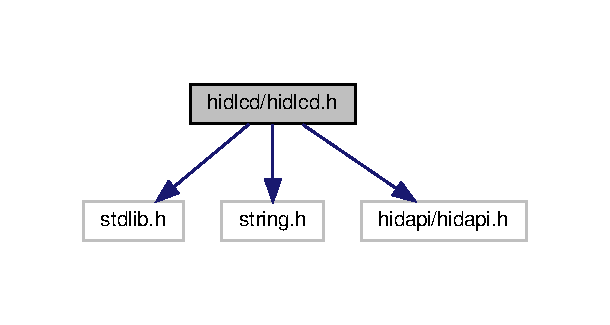
\includegraphics[width=293pt]{hidlcd_8h__incl}
\end{center}
\end{figure}
\subsection*{Classes}
\begin{DoxyCompactItemize}
\item 
struct \hyperlink{structHIDDisplayParams}{H\+I\+D\+Display\+Params}
\begin{DoxyCompactList}\small\item\em The structure holding the physical parameters and other capabilities of the L\+CD display. \end{DoxyCompactList}\end{DoxyCompactItemize}
\subsection*{Macros}
\begin{DoxyCompactItemize}
\item 
\mbox{\Hypertarget{hidlcd_8h_a5042d962440a29403f991f980f208e41}\label{hidlcd_8h_a5042d962440a29403f991f980f208e41}} 
\#define \hyperlink{hidlcd_8h_a5042d962440a29403f991f980f208e41}{H\+I\+D\+\_\+\+A\+U\+X\+D\+\_\+\+D\+I\+S\+P\+L\+A\+Y\+\_\+\+P\+A\+R\+A\+MS}~0x01
\begin{DoxyCompactList}\small\item\em Display parameters report. \end{DoxyCompactList}\item 
\mbox{\Hypertarget{hidlcd_8h_ab44584556ff0122c2be007658ae49837}\label{hidlcd_8h_ab44584556ff0122c2be007658ae49837}} 
\#define \hyperlink{hidlcd_8h_ab44584556ff0122c2be007658ae49837}{H\+I\+D\+\_\+\+A\+U\+X\+D\+\_\+\+C\+U\+R\+S\+O\+R\+\_\+\+P\+OS}~0x02
\begin{DoxyCompactList}\small\item\em Cursor position report. \end{DoxyCompactList}\item 
\mbox{\Hypertarget{hidlcd_8h_abbafade9596c65093964384e7eb1c46f}\label{hidlcd_8h_abbafade9596c65093964384e7eb1c46f}} 
\#define \hyperlink{hidlcd_8h_abbafade9596c65093964384e7eb1c46f}{H\+I\+D\+\_\+\+A\+U\+X\+D\+\_\+\+C\+H\+A\+R\+\_\+\+R\+E\+P\+O\+RT}~0x03
\begin{DoxyCompactList}\small\item\em Character report. \end{DoxyCompactList}\item 
\mbox{\Hypertarget{hidlcd_8h_aa291f31293728a2fac1cdaa837c2f175}\label{hidlcd_8h_aa291f31293728a2fac1cdaa837c2f175}} 
\#define \hyperlink{hidlcd_8h_aa291f31293728a2fac1cdaa837c2f175}{H\+I\+D\+\_\+\+A\+U\+X\+D\+\_\+\+F\+O\+N\+T\+\_\+\+R\+E\+P\+O\+RT}~0x04
\begin{DoxyCompactList}\small\item\em Font report. \end{DoxyCompactList}\item 
\mbox{\Hypertarget{hidlcd_8h_aad7ed55b46dd30f39b9ad4496641ba60}\label{hidlcd_8h_aad7ed55b46dd30f39b9ad4496641ba60}} 
\#define \hyperlink{hidlcd_8h_aad7ed55b46dd30f39b9ad4496641ba60}{H\+I\+D\+\_\+\+A\+U\+X\+D\+\_\+\+C\+T\+R\+L\+\_\+\+R\+E\+P\+O\+RT}~0x05
\begin{DoxyCompactList}\small\item\em Control report. \end{DoxyCompactList}\item 
\mbox{\Hypertarget{hidlcd_8h_af89b3f11d1fdc5d558f36e38de08813a}\label{hidlcd_8h_af89b3f11d1fdc5d558f36e38de08813a}} 
\#define \hyperlink{hidlcd_8h_af89b3f11d1fdc5d558f36e38de08813a}{H\+I\+D\+\_\+\+A\+U\+X\+D\+\_\+\+C\+U\+R\+S\+O\+R\+\_\+\+F\+L\+A\+GS}~0x06
\begin{DoxyCompactList}\small\item\em Control report. \end{DoxyCompactList}\item 
\mbox{\Hypertarget{hidlcd_8h_a11ed1c8885387fcaef425ec16bf8f6d1}\label{hidlcd_8h_a11ed1c8885387fcaef425ec16bf8f6d1}} 
\#define \hyperlink{hidlcd_8h_a11ed1c8885387fcaef425ec16bf8f6d1}{H\+I\+D\+\_\+\+A\+U\+X\+D\+\_\+\+A\+S\+C\+I\+I\+\_\+\+C\+H\+A\+R\+S\+ET}~0x80
\begin{DoxyCompactList}\small\item\em Screen supports. \end{DoxyCompactList}\item 
\mbox{\Hypertarget{hidlcd_8h_af446a9f6100bbbfdbd221da903c51c20}\label{hidlcd_8h_af446a9f6100bbbfdbd221da903c51c20}} 
\#define \hyperlink{hidlcd_8h_af446a9f6100bbbfdbd221da903c51c20}{H\+I\+D\+\_\+\+A\+U\+X\+D\+\_\+\+D\+A\+T\+A\+R\+E\+A\+D\+\_\+\+B\+A\+CK}~0x40
\begin{DoxyCompactList}\small\item\em Character Report can be read back when set. \end{DoxyCompactList}\item 
\mbox{\Hypertarget{hidlcd_8h_aaf12661f504f60b04e0d10841c9a208d}\label{hidlcd_8h_aaf12661f504f60b04e0d10841c9a208d}} 
\#define \hyperlink{hidlcd_8h_aaf12661f504f60b04e0d10841c9a208d}{H\+I\+D\+\_\+\+A\+U\+X\+D\+\_\+\+F\+O\+N\+T\+R\+E\+A\+D\+\_\+\+B\+A\+CK}~0x20
\begin{DoxyCompactList}\small\item\em Font Report can be read back when set. \end{DoxyCompactList}\item 
\mbox{\Hypertarget{hidlcd_8h_acbe50d5d58ea5f5e976daa7b82f3c54b}\label{hidlcd_8h_acbe50d5d58ea5f5e976daa7b82f3c54b}} 
\#define \hyperlink{hidlcd_8h_acbe50d5d58ea5f5e976daa7b82f3c54b}{H\+I\+D\+\_\+\+A\+U\+X\+D\+\_\+\+C\+L\+E\+AR}~0x80
\begin{DoxyCompactList}\small\item\em Clear Display command. \end{DoxyCompactList}\item 
\mbox{\Hypertarget{hidlcd_8h_a9c91cbfb06dd384e2619429d7bb22b8f}\label{hidlcd_8h_a9c91cbfb06dd384e2619429d7bb22b8f}} 
\#define \hyperlink{hidlcd_8h_a9c91cbfb06dd384e2619429d7bb22b8f}{H\+I\+D\+\_\+\+A\+U\+X\+D\+\_\+\+E\+N\+A\+B\+LE}~0x40
\begin{DoxyCompactList}\small\item\em Display enable. \end{DoxyCompactList}\item 
\mbox{\Hypertarget{hidlcd_8h_aaebadc19a66a24350172e32cbb29fadd}\label{hidlcd_8h_aaebadc19a66a24350172e32cbb29fadd}} 
\#define \hyperlink{hidlcd_8h_aaebadc19a66a24350172e32cbb29fadd}{H\+I\+D\+\_\+\+A\+U\+X\+D\+\_\+\+S\+S\+E\+N\+A\+B\+LE}~0x20
\begin{DoxyCompactList}\small\item\em Screen Saver enable. \end{DoxyCompactList}\item 
\mbox{\Hypertarget{hidlcd_8h_a04cd720fad303bfee7402eb929db9d2c}\label{hidlcd_8h_a04cd720fad303bfee7402eb929db9d2c}} 
\#define \hyperlink{hidlcd_8h_a04cd720fad303bfee7402eb929db9d2c}{H\+I\+D\+\_\+\+A\+U\+X\+D\+\_\+\+V\+S\+C\+R\+O\+LL}~0x10
\begin{DoxyCompactList}\small\item\em Vertical Scroll. \end{DoxyCompactList}\item 
\mbox{\Hypertarget{hidlcd_8h_ae1273eeaeed3bed194f227577419ac7a}\label{hidlcd_8h_ae1273eeaeed3bed194f227577419ac7a}} 
\#define \hyperlink{hidlcd_8h_ae1273eeaeed3bed194f227577419ac7a}{H\+I\+D\+\_\+\+A\+U\+X\+D\+\_\+\+H\+S\+C\+R\+O\+LL}~0x08
\begin{DoxyCompactList}\small\item\em Horizintal Scroll. \end{DoxyCompactList}\item 
\mbox{\Hypertarget{hidlcd_8h_a9ca983345d847d128e52d03f19fd81b5}\label{hidlcd_8h_a9ca983345d847d128e52d03f19fd81b5}} 
\#define \hyperlink{hidlcd_8h_a9ca983345d847d128e52d03f19fd81b5}{H\+I\+D\+\_\+\+A\+U\+X\+D\+\_\+\+D\+I\+S\+A\+B\+LE}~0x0
\begin{DoxyCompactList}\small\item\em Display disable. \end{DoxyCompactList}\item 
\mbox{\Hypertarget{hidlcd_8h_ab1874afc9cbb34febd4fbc780d7180de}\label{hidlcd_8h_ab1874afc9cbb34febd4fbc780d7180de}} 
\#define \hyperlink{hidlcd_8h_ab1874afc9cbb34febd4fbc780d7180de}{H\+I\+D\+\_\+\+A\+D\+C\+M\+D\+\_\+\+M\+O\+D\+E\+\_\+\+D\+E\+F\+A\+U\+LT}~0x0
\begin{DoxyCompactList}\small\item\em Command flags are added to the existing state of screen. \end{DoxyCompactList}\item 
\mbox{\Hypertarget{hidlcd_8h_a0cc7c1efd85b98deea98dc7ba6be892f}\label{hidlcd_8h_a0cc7c1efd85b98deea98dc7ba6be892f}} 
\#define \hyperlink{hidlcd_8h_a0cc7c1efd85b98deea98dc7ba6be892f}{H\+I\+D\+\_\+\+A\+D\+C\+M\+D\+\_\+\+M\+O\+D\+E\+\_\+\+O\+FF}~0x1
\begin{DoxyCompactList}\small\item\em Clear the command/state. \end{DoxyCompactList}\item 
\mbox{\Hypertarget{hidlcd_8h_ab033c7a7187b9974b0adb1edcf0f76b1}\label{hidlcd_8h_ab033c7a7187b9974b0adb1edcf0f76b1}} 
\#define \hyperlink{hidlcd_8h_ab033c7a7187b9974b0adb1edcf0f76b1}{H\+I\+D\+\_\+\+A\+D\+C\+M\+D\+\_\+\+M\+O\+D\+E\+\_\+\+O\+V\+E\+R\+W\+R\+I\+TE}~0x2
\begin{DoxyCompactList}\small\item\em Ovewrite the state of the screen. \end{DoxyCompactList}\item 
\mbox{\Hypertarget{hidlcd_8h_a4087c655e349b29254aeacf47f96d479}\label{hidlcd_8h_a4087c655e349b29254aeacf47f96d479}} 
\#define \hyperlink{hidlcd_8h_a4087c655e349b29254aeacf47f96d479}{H\+I\+D\+\_\+\+A\+D\+C\+C\+\_\+\+P\+I\+X\+E\+L\+P\+OS}~0x80
\begin{DoxyCompactList}\small\item\em Cursor Pixel Positioning. \end{DoxyCompactList}\item 
\mbox{\Hypertarget{hidlcd_8h_ab35eebcd769df894de1058d8efed22e3}\label{hidlcd_8h_ab35eebcd769df894de1058d8efed22e3}} 
\#define \hyperlink{hidlcd_8h_ab35eebcd769df894de1058d8efed22e3}{H\+I\+D\+\_\+\+A\+D\+C\+C\+\_\+\+I\+N\+C\+R\+E\+M\+E\+NT}~0x40
\begin{DoxyCompactList}\small\item\em Cursor Mode = Increment. \end{DoxyCompactList}\item 
\mbox{\Hypertarget{hidlcd_8h_affab81d7aff670596c70004116280341}\label{hidlcd_8h_affab81d7aff670596c70004116280341}} 
\#define \hyperlink{hidlcd_8h_affab81d7aff670596c70004116280341}{H\+I\+D\+\_\+\+A\+D\+C\+C\+\_\+\+E\+N\+A\+B\+LE}~0x20
\begin{DoxyCompactList}\small\item\em Cursor Enable. \end{DoxyCompactList}\item 
\mbox{\Hypertarget{hidlcd_8h_a13005b68e705d0033f93d069156a656a}\label{hidlcd_8h_a13005b68e705d0033f93d069156a656a}} 
\#define \hyperlink{hidlcd_8h_a13005b68e705d0033f93d069156a656a}{H\+I\+D\+\_\+\+A\+D\+C\+C\+\_\+\+B\+L\+I\+NK}~0x10
\begin{DoxyCompactList}\small\item\em Cursor Blink. \end{DoxyCompactList}\end{DoxyCompactItemize}
\subsection*{Functions}
\begin{DoxyCompactItemize}
\item 
\hyperlink{structHIDDisplayParams}{H\+I\+D\+Display\+Params} $\ast$H\+I\+D\+\_\+\+A\+P\+I\+\_\+\+E\+X\+P\+O\+RT H\+I\+D\+\_\+\+A\+P\+I\+\_\+\+C\+A\+LL \hyperlink{group__API_gabb41034a653433cec87bd56d20e7da32}{hidlcd\+\_\+get\+\_\+display\+\_\+params} (hid\+\_\+device $\ast$dev)
\begin{DoxyCompactList}\small\item\em Returns the physical parameters of the connected auxiliary L\+CD display. \end{DoxyCompactList}\item 
H\+I\+D\+\_\+\+A\+P\+I\+\_\+\+E\+X\+P\+O\+RT hid\+\_\+device $\ast$H\+I\+D\+\_\+\+A\+P\+I\+\_\+\+C\+A\+LL \hyperlink{group__API_ga9fbc6a6acff713baca89139cc99fed1e}{hidlcd\+\_\+open} (unsigned short vendor\+\_\+id, unsigned short product\+\_\+id, const wchar\+\_\+t $\ast$serial\+\_\+number)
\begin{DoxyCompactList}\small\item\em Returns the device handle. \end{DoxyCompactList}\item 
void H\+I\+D\+\_\+\+A\+P\+I\+\_\+\+E\+X\+P\+O\+RT H\+I\+D\+\_\+\+A\+P\+I\+\_\+\+C\+A\+LL \hyperlink{group__API_gab5076b4a075677b9298c2261621668bf}{hidlcd\+\_\+close} (hid\+\_\+device $\ast$dev)
\begin{DoxyCompactList}\small\item\em Closes the device handle and releases associated resources. \end{DoxyCompactList}\item 
int H\+I\+D\+\_\+\+A\+P\+I\+\_\+\+E\+X\+P\+O\+RT H\+I\+D\+\_\+\+A\+P\+I\+\_\+\+C\+A\+LL \hyperlink{group__API_ga67748e0754a894b7d04d9f0beef058fc}{hidlcd\+\_\+exit} (void)
\begin{DoxyCompactList}\small\item\em Closes the H\+I\+D\+L\+CD library and releases associated resources. \end{DoxyCompactList}\item 
int H\+I\+D\+\_\+\+A\+P\+I\+\_\+\+E\+X\+P\+O\+RT H\+I\+D\+\_\+\+A\+P\+I\+\_\+\+C\+A\+LL \hyperlink{group__API_ga37c732d4d14ea4584ee33e6e258deba7}{hidlcd\+\_\+init} (void)
\begin{DoxyCompactList}\small\item\em Initialize the H\+I\+D\+L\+CD library. \end{DoxyCompactList}\item 
int H\+I\+D\+\_\+\+A\+P\+I\+\_\+\+E\+X\+P\+O\+RT H\+I\+D\+\_\+\+A\+P\+I\+\_\+\+C\+A\+LL \hyperlink{group__API_ga0c27c33eef05230a5ed6e1d6ea6cb489}{hidlcd\+\_\+set\+\_\+cursor} (hid\+\_\+device $\ast$dev, u\+\_\+int8\+\_\+t row, u\+\_\+int8\+\_\+t col)
\begin{DoxyCompactList}\small\item\em This function sets the cursor of the L\+CD display in the specified position. \end{DoxyCompactList}\item 
int H\+I\+D\+\_\+\+A\+P\+I\+\_\+\+E\+X\+P\+O\+RT H\+I\+D\+\_\+\+A\+P\+I\+\_\+\+C\+A\+LL \hyperlink{group__API_gae33cb27bbbe1ae372fd3b98f16bd665d}{hidlcd\+\_\+set\+\_\+cursor\+\_\+flags\+\_\+ext} (hid\+\_\+device $\ast$dev, u\+\_\+int8\+\_\+t flags, u\+\_\+int8\+\_\+t mode)
\begin{DoxyCompactList}\small\item\em This function sets the cursor extended parameters and display mode. \end{DoxyCompactList}\item 
int H\+I\+D\+\_\+\+A\+P\+I\+\_\+\+E\+X\+P\+O\+RT H\+I\+D\+\_\+\+A\+P\+I\+\_\+\+C\+A\+LL \hyperlink{group__API_gab5c3e5de5b25ce048739fb5570fceabc}{hidlcd\+\_\+print} (hid\+\_\+device $\ast$dev, \hyperlink{structHIDDisplayParams}{H\+I\+D\+Display\+Params} $\ast$display\+\_\+params, const char $\ast$string)
\begin{DoxyCompactList}\small\item\em Prints the text on the L\+CD screen. \end{DoxyCompactList}\item 
int H\+I\+D\+\_\+\+A\+P\+I\+\_\+\+E\+X\+P\+O\+RT H\+I\+D\+\_\+\+A\+P\+I\+\_\+\+C\+A\+LL \hyperlink{group__API_gad6c000babbc378230a1a7023bd53b8b2}{hidlcd\+\_\+send\+\_\+command\+\_\+ext} (hid\+\_\+device $\ast$dev, u\+\_\+int8\+\_\+t command, u\+\_\+int8\+\_\+t mode)
\begin{DoxyCompactList}\small\item\em Sends the command to the L\+CD display with mode. \end{DoxyCompactList}\item 
int H\+I\+D\+\_\+\+A\+P\+I\+\_\+\+E\+X\+P\+O\+RT H\+I\+D\+\_\+\+A\+P\+I\+\_\+\+C\+A\+LL \hyperlink{group__API_ga1ec7653ee073e917475c01ee9e1252e4}{hidlcd\+\_\+send\+\_\+command} (hid\+\_\+device $\ast$dev, u\+\_\+int8\+\_\+t command)
\begin{DoxyCompactList}\small\item\em Sends the command to the L\+CD display. \end{DoxyCompactList}\end{DoxyCompactItemize}


\subsection{Detailed Description}
\begin{DoxyAuthor}{Author}
Alex Bratchik 
\end{DoxyAuthor}

%--- End generated contents ---

% Index
\backmatter
\newpage
\phantomsection
\clearemptydoublepage
\addcontentsline{toc}{chapter}{Index}
\printindex

\end{document}
